\subsection{Ist-Analyse}
\label{sec:IstAnalyse}

Momentan lassen sich Informationen über die angebotenen Studiengänge am Studien-
standort Lingen über die Hochschulseite www.hs-osnabrueck.de abrufen. Die Internetseite bietet dabei zum einen 
weiterführende Links zu den einzelnen Instituten und darüber auch viele Informationen für Unternehmen und Studierende.
Hier werden zum Beispiel Labore, Projekte und Dozenten der einezelnen Institute vorgestellt. Zum anderen werden in einer 
Bildergalerie einzelne Impressionen des neuen Campus dargestellt. Ein Screenshot hiervon ist in Abbildung 2 (Aktuelle 
Informationsseite über den Campus in Lingen) abgebildet.

\begin{figure}[htb]
\centering
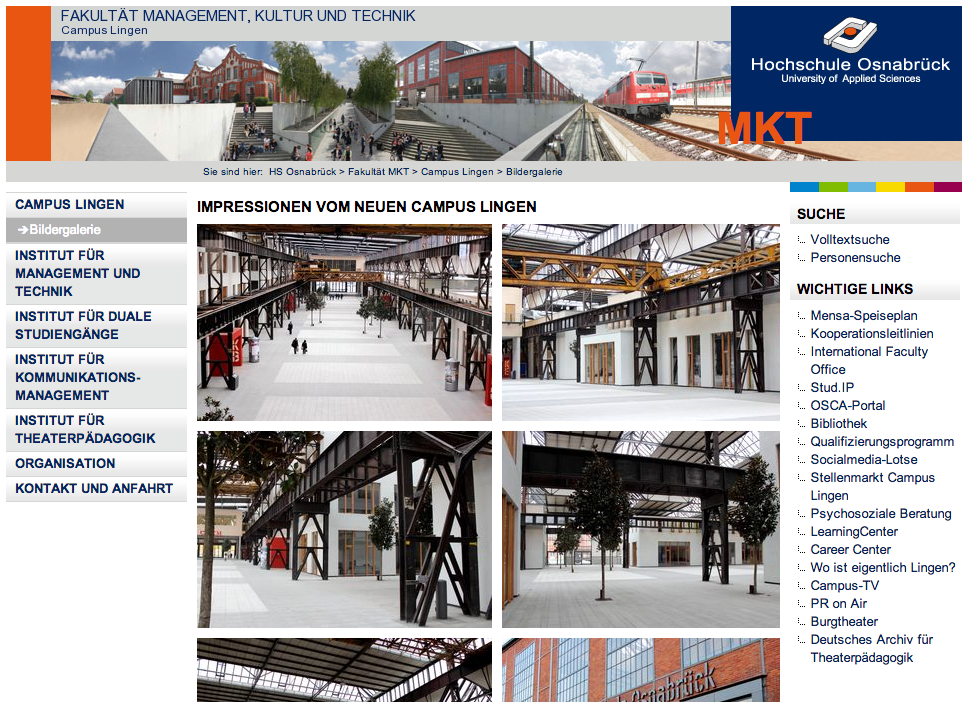
\includegraphics[width=1.0\textwidth]{Bildergalerie.png}
\caption[Campus Lingen Bildergalerie]{Bildergaliere des Campus Lingen\protect\footnotemark}
\label{fig:Architektur}
\end{figure}
\footnotetext{\url: http://www.campus-lingen.hs-osnabrueck.de}

Ähnlich wie die Informationsvermittlung auf der Internetseite der Hochschule Osnabrück
gestaltet sich auch die Informationsvermittlung auf Messen, auf denen Studieninteressierte
sich auch über die einzelnen Studienstandorte erkundigen können. Dort werden ebenfalls
Impressionen des Campus in Lingen gezeigt oder Informationsmaterial verteilt.

Vor dem Hintergrund der Projektidee, den Campus in 360-Grad Panoramas mit Informationstexten abzubilden, bilden sich aus 
dieser Analyse 2 interessante Elemente heraus.

\textbf{1.} Die Fotos, die bereits vom neuen Campus gemacht wurden.

\textbf{2.} Das Informationsmaterial das über Projekte, Studiengänge, Dozenten und weiteres zusammen getragen wurde.

Die bereits angefertigen Fotos können dabei nicht für das vorliegende Projekt verwendet werden, da es sich bei diesen 
Fotos nicht um 360-Grad Panoramafotos handelt. Darüber hinaus sind auf diesen Fotos nur einzelne Impressionen des Campus 
dargestellt. Das bedeutet die bestehenden Fotos müssten um neu angefertigte ergänzt werden und das ist aus Gründen 
unterschiedlicher Lichterverhältnisse kein sinnvolles Vorgehen. Die bestehenden Impressionen geben aber ein Einblick in 
interessante Blickwickel auf den Campus. Diese Blickwinkel können bei der Erstellung der neuen Fotos aufgeriffen werden. 

Das zusammengetragene Informationsmaterial kann dagegen aus der Internetquelle der Hochschule verwendet werden, um 
Informationen zu bestimmten Panoramas anzuzeigen. Für die Rechereche nach Informationsmaterial muss daher kein weiter 
Aufwand im Projekt berücksichtigt werden.